% Adjust these for the path of the theme and its graphics, relative to this file
%\usepackage{beamerthemeFalmouthGamesAcademy}
\usepackage{../../beamerthemeFalmouthGamesAcademy}
\usepackage{multimedia}
\graphicspath{ {../../} }

% Default language for code listings
\lstset{language=C++,
        morekeywords={each,in,nullptr}
}

% For strikethrough effect
\usepackage[normalem]{ulem}
\usepackage{wasysym}

\usepackage{pdfpages}

% http://www.texample.net/tikz/examples/state-machine/
\usetikzlibrary{arrows,automata}

\newcommand{\modulecode}{COMP260}\newcommand{\moduletitle}{Distributed Systems}\newcommand{\sessionnumber}{5}

\begin{document}
\title{\sessionnumber: Session title here}
\subtitle{\modulecode: \moduletitle}

\frame{\titlepage} 

\begin{frame}
	\frametitle{Learning outcomes}
	\begin{itemize}
		\item \textbf{Recognise} how audio is used in games
		\item \textbf{Explain} what sound is and how it can be represented digitally
		\item \textbf{Write} a program that will produce a sound
	\end{itemize}
\end{frame}

\part{Introduction}
\frame{\partpage}

\begin{frame}{What is Post-Processing?}
	\begin{itemize}
		\pause\item Is a series of techniques that are carried out after a scene has been rendered
		\pause\item Traditionally this could only be done as an offline process
		\pause\item With the advent of faster GPUs and programmable shaders, we could implement some of the effects in real time
		\pause\item The key to the effect is to switch from drawing to the back buffer to a texture
		\pause\item This texture will contain the scene
		\pause\item We then use a shader to implement a post-processing effect
		\pause\item We then map the processed texture onto a full screen quad, which is rendered to the backbuffer
	\end{itemize}
\end{frame}
\part{How are sounds used in Games?}
\frame{\partpage}

\begin{frame}{Audio in Games}

\begin{center}
	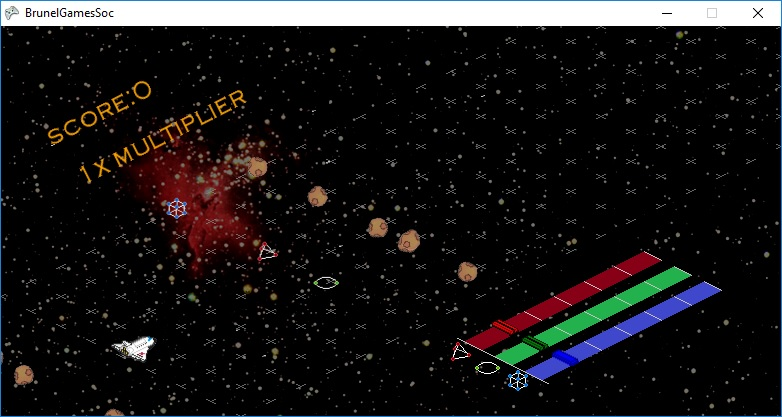
\includegraphics[width=\linewidth,height=0.8\textheight,keepaspectratio]{astroclysm}

	\vspace{1em}

	Astroclysm - X48 2008
\end{center}

\end{frame}

\begin{frame}{Audio in Games}

\begin{center}
	\url{https://www.youtube.com/watch?v=oF7POPv1GyQ}

	\vspace{1em}
		
	\url{https://www.dropbox.com/sh/vrodjzp0zerimik/AAA_OScznYHq9HWgoP0p0K2wa?dl=1}	
\end{center}

\end{frame}

\begin{frame}{Audio in Games}

\begin{itemize}
	\item For the next 10 mins, in pairs:
	\begin{itemize}
		\item Discuss one or two games that use sounds in an interesting way
		\item What was interesting about the use?
	\end{itemize}
\end{itemize}

\end{frame}
\part{What is sound? What is a wave?}
\frame{\partpage}

\begin{frame}
	\begin{center}
		\textbf{Quick Definition:} A wave of compression and refraction in an elastic medium, such as air, which can be detected by an animal’s sense of hearing 
	\end{center}
\end{frame}

\begin{frame}{What is Sound?}
	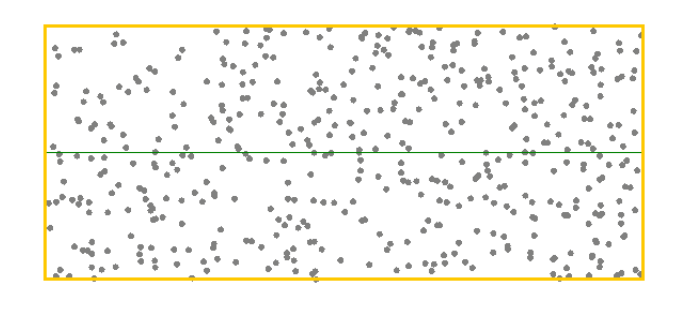
\includegraphics[width=\linewidth,height=0.8\textheight,keepaspectratio]{sound_molecules}
\end{frame}

\begin{frame}{What is a Wave?}
	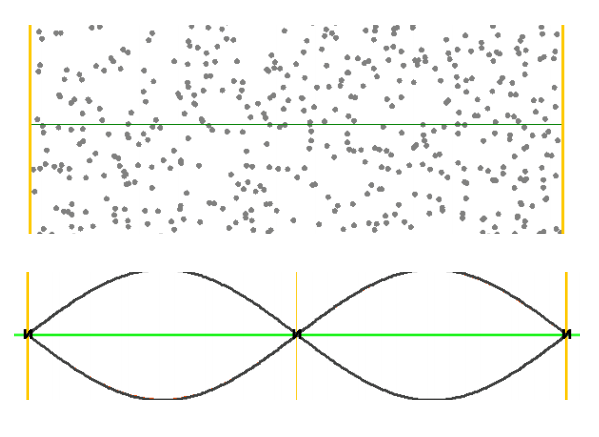
\includegraphics[width=\linewidth,height=0.8\textheight,keepaspectratio]{sound_wave}
\end{frame}

\begin{frame}{What is a Wave?}
	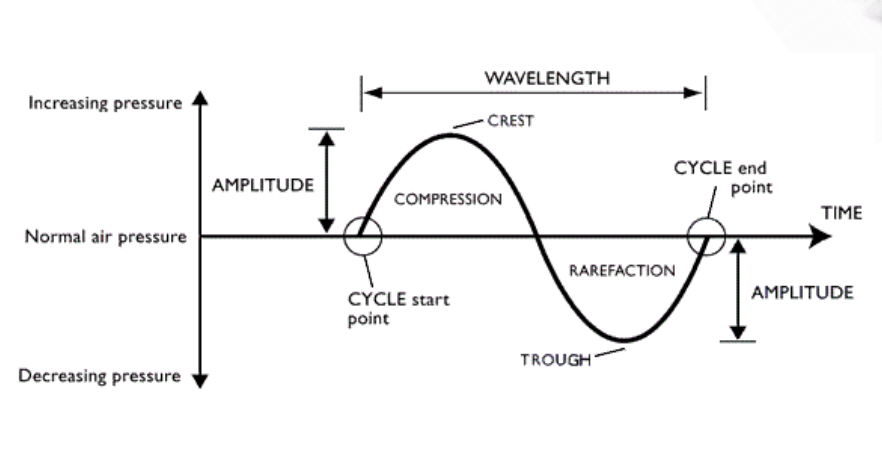
\includegraphics[width=\linewidth,height=0.8\textheight,keepaspectratio]{wave_desc}
\end{frame}

\begin{frame}{What is Sound?}
	\begin{itemize}
		\item Many animals are able to sense sound in two key ways:
		\textbf{volume} and \textbf{pitch}.
		\item\textbf{Volume:} The intensity of the change in pressure, as signified by the
		amplitude of a wave
		\item\textbf{Pitch:} The frequency of the change, as signified by the length of
		the wave and its velocity (i.e., “the speed of sound”)
	\end{itemize}
\end{frame}

\end{document}
